\begin{anexosenv}

\partanexos

\chapter{Análise dos Percentis do Estudo de Caso} \label{anex:percentis}

Neste anexo contém os gráficos relacionados com a análise de percentis de cada
uma das métricas de vulnerabilidades apresentadas em \ref{cap:metricas_vuln}
do
projeto Linux, sendo esses parte dos resultados descritos na seção \ref{analise_estudo}.


\begin{figure}[h]
  \centering
  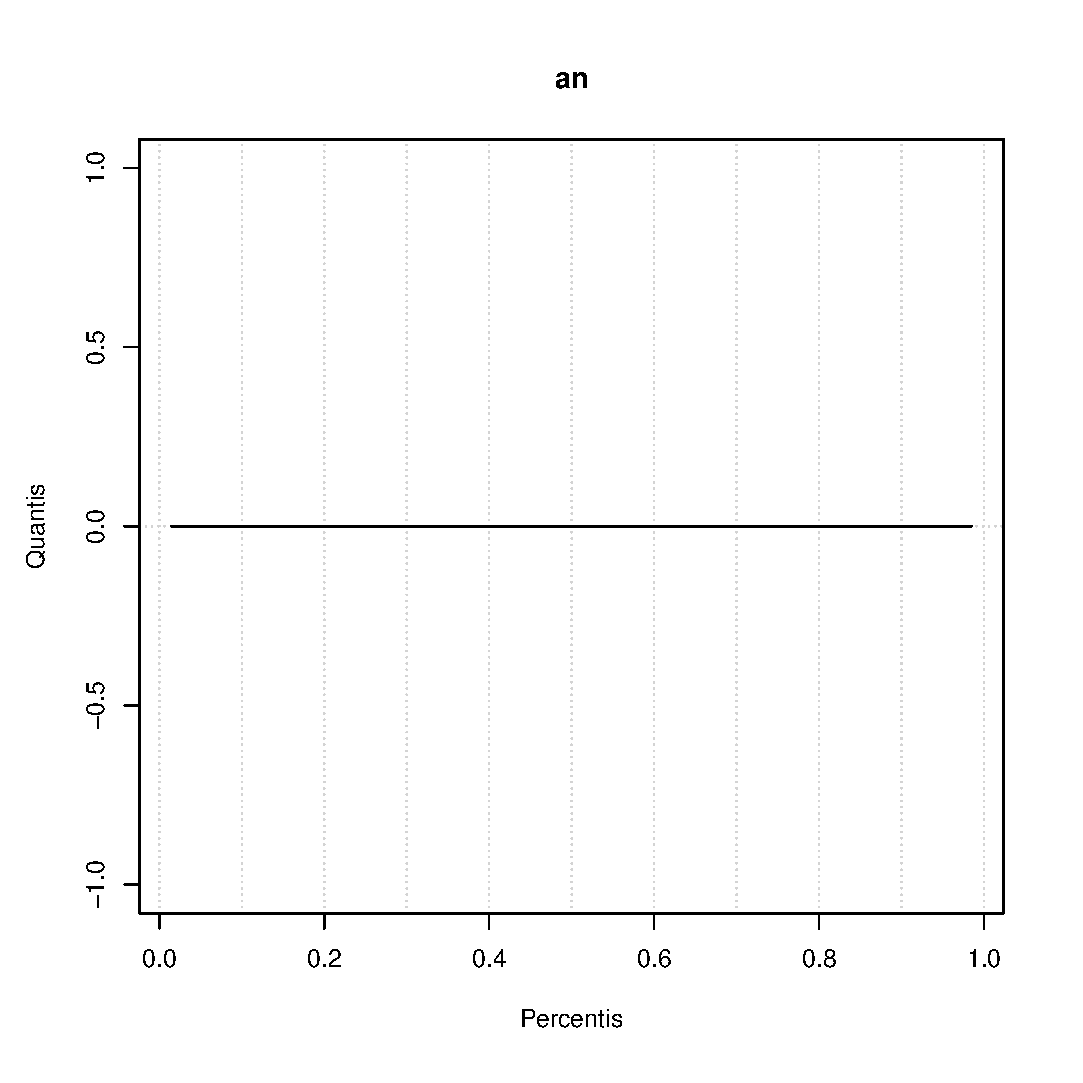
\includegraphics[width=0.7\textwidth]
      {dados/linux/an.eps}
  \caption{Gráfico de Percentis da métrica AN}
\end{figure}

\newpage

\begin{figure}[h]
  \centering
  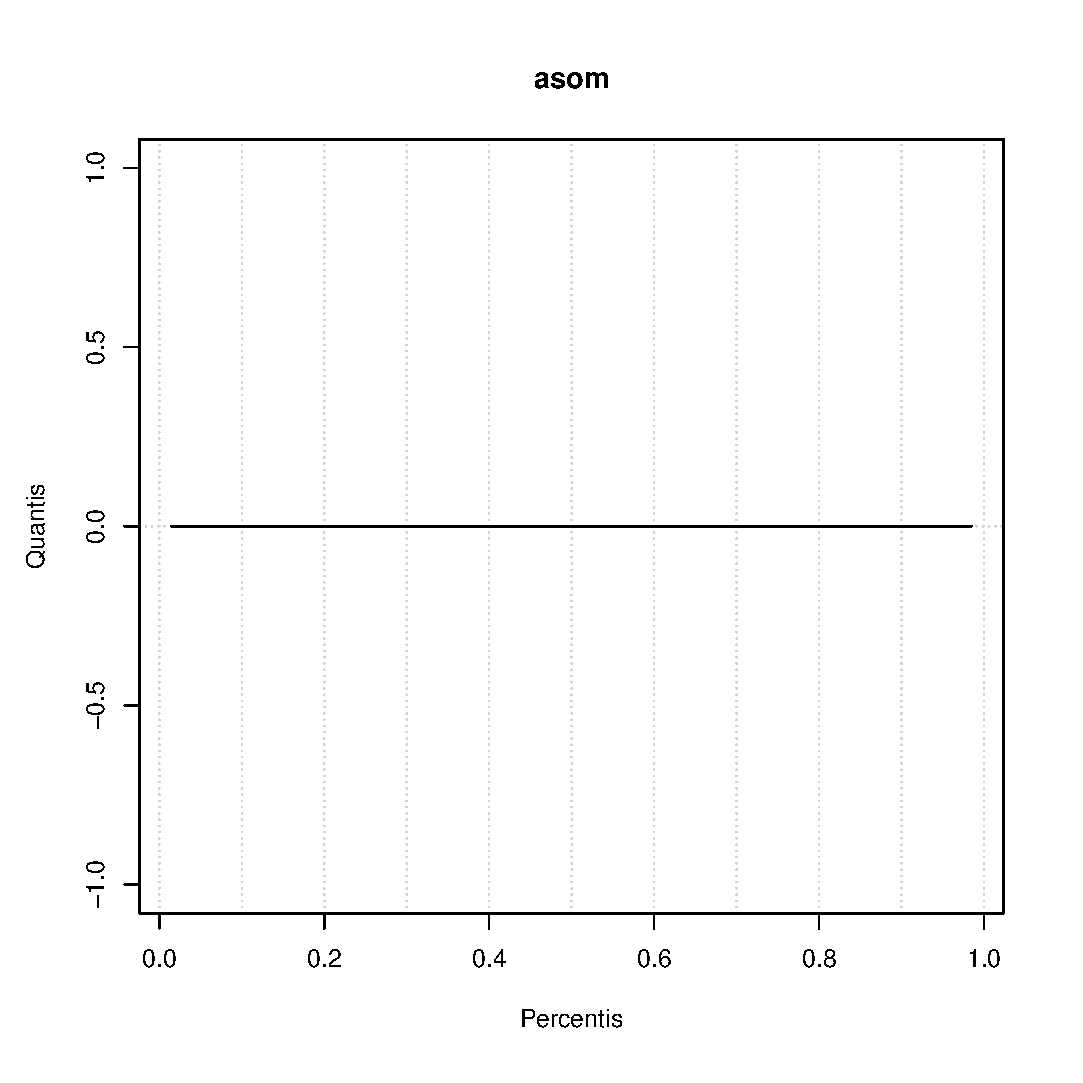
\includegraphics[width=0.6\textwidth]
      {dados/linux/asom.eps}
  \caption{Gráfico de Percentis da métrica ASOM}
  \label{graphic:asom}
\end{figure}

\begin{figure}[h]
  \centering
  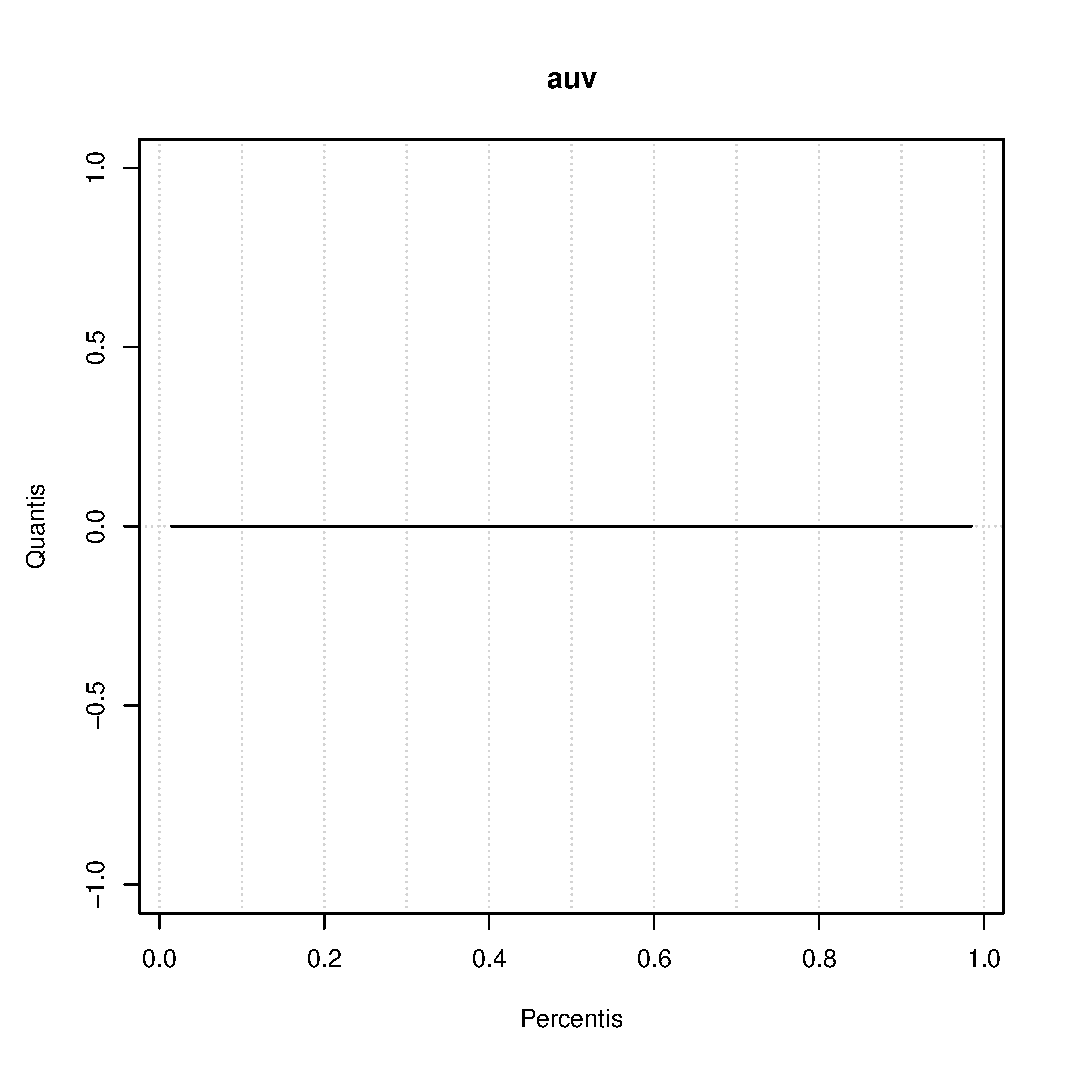
\includegraphics[width=0.6\textwidth]
      {dados/linux/auv.eps}
  \caption{Gráfico de Percentis da métrica AUV}
\end{figure}

\newpage

\begin{figure}[h]
  \centering
  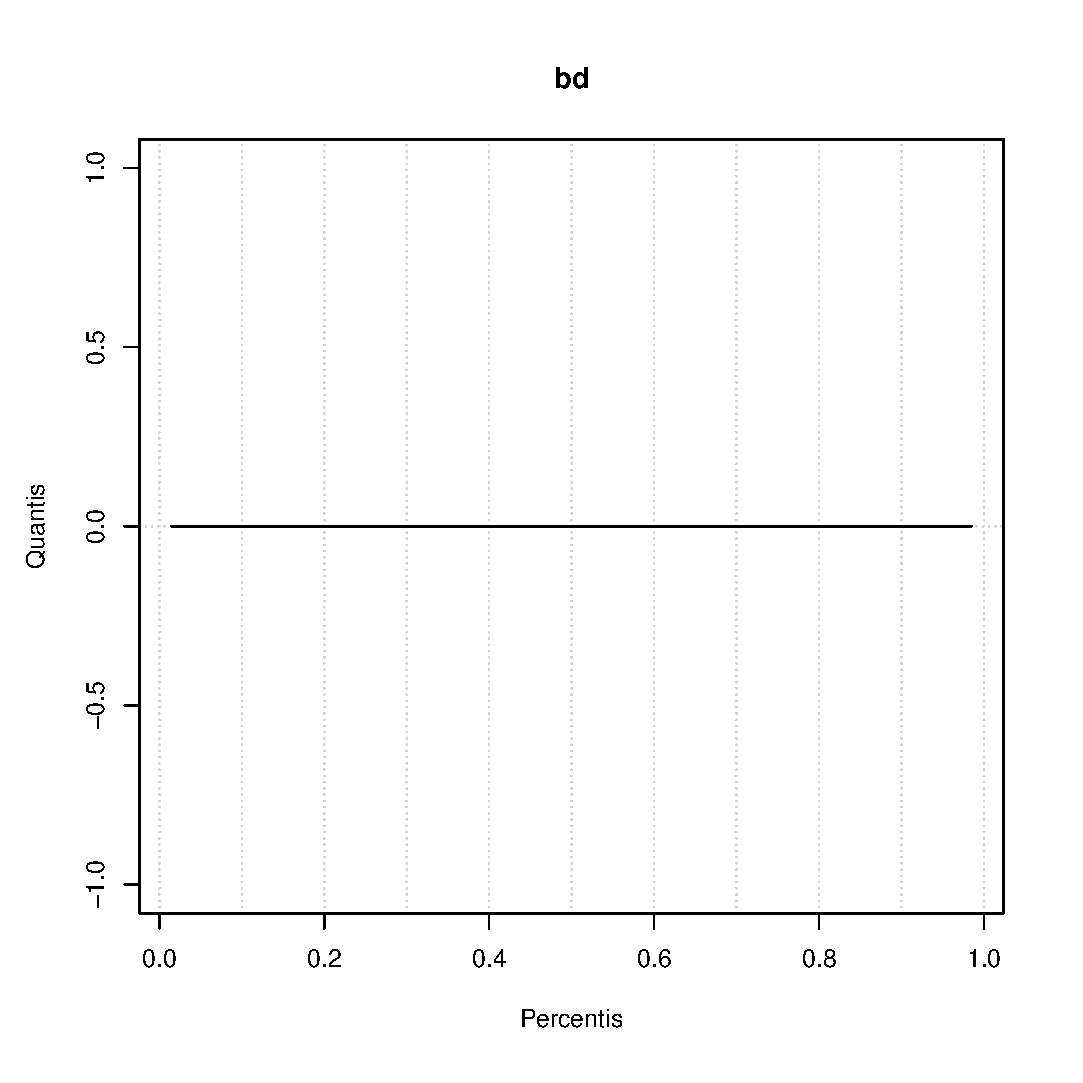
\includegraphics[width=0.6\textwidth]
      {dados/linux/bd.eps}
  \caption{Gráfico de Percentis da métrica BD}
\end{figure}

\begin{figure}[h]
  \centering
  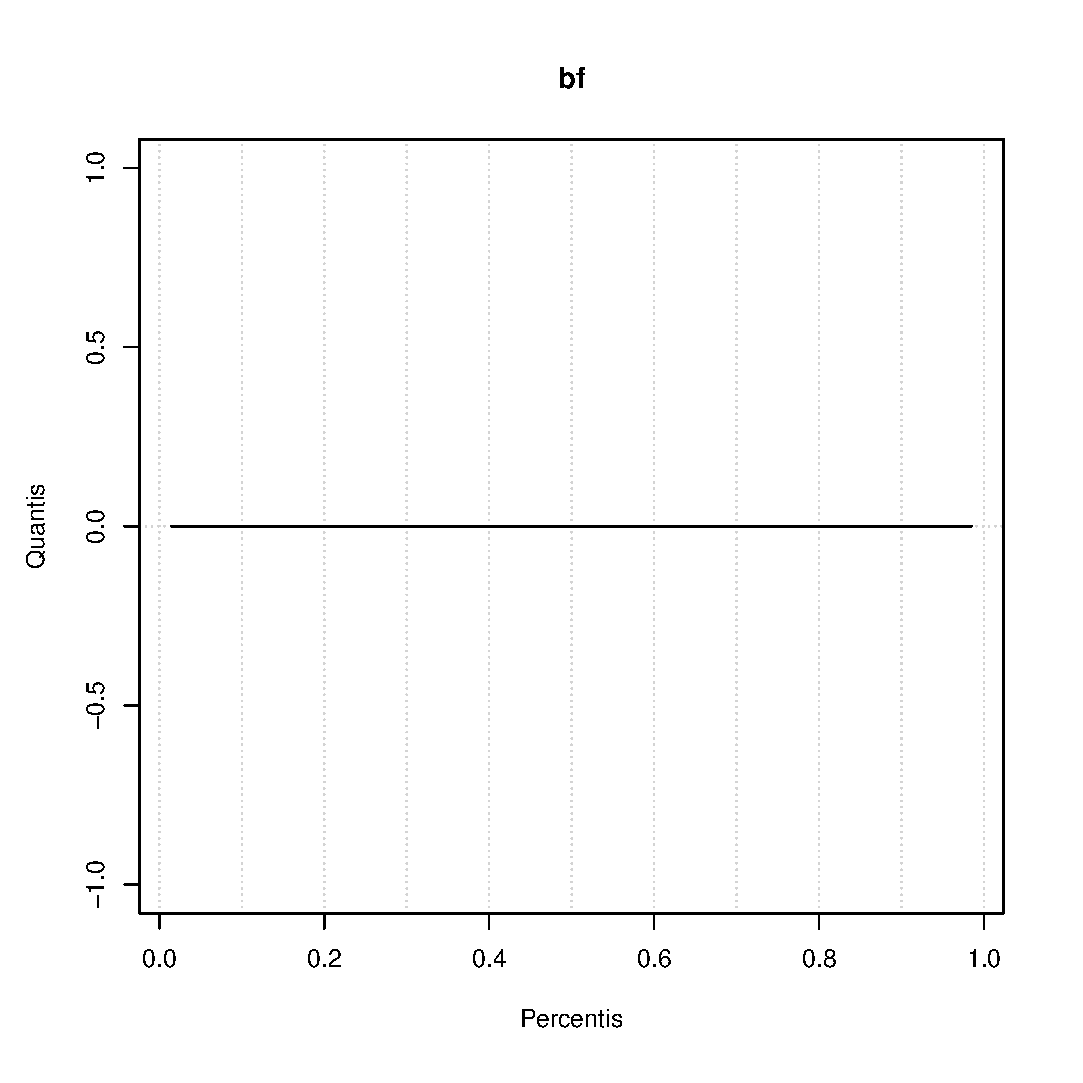
\includegraphics[width=0.6\textwidth]
      {dados/linux/bf.eps}
  \caption{Gráfico de Percentis da métrica BF}
\end{figure}

\newpage

\begin{figure}[h]
  \centering
  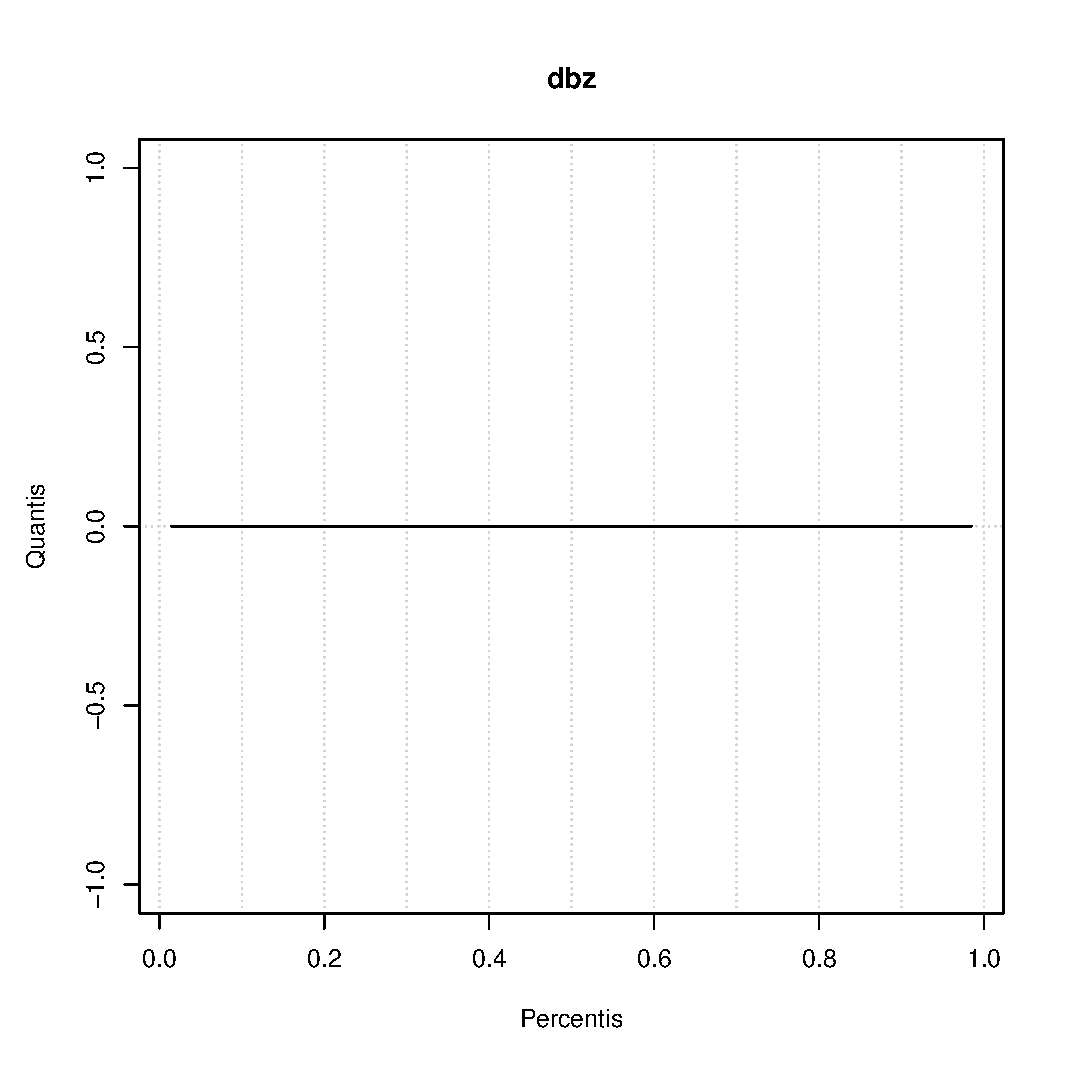
\includegraphics[width=0.6\textwidth]
      {dados/linux/dbz.eps}
  \caption{Gráfico de Percentis da métrica DBZ}
\end{figure}

\begin{figure}[h]
  \centering
  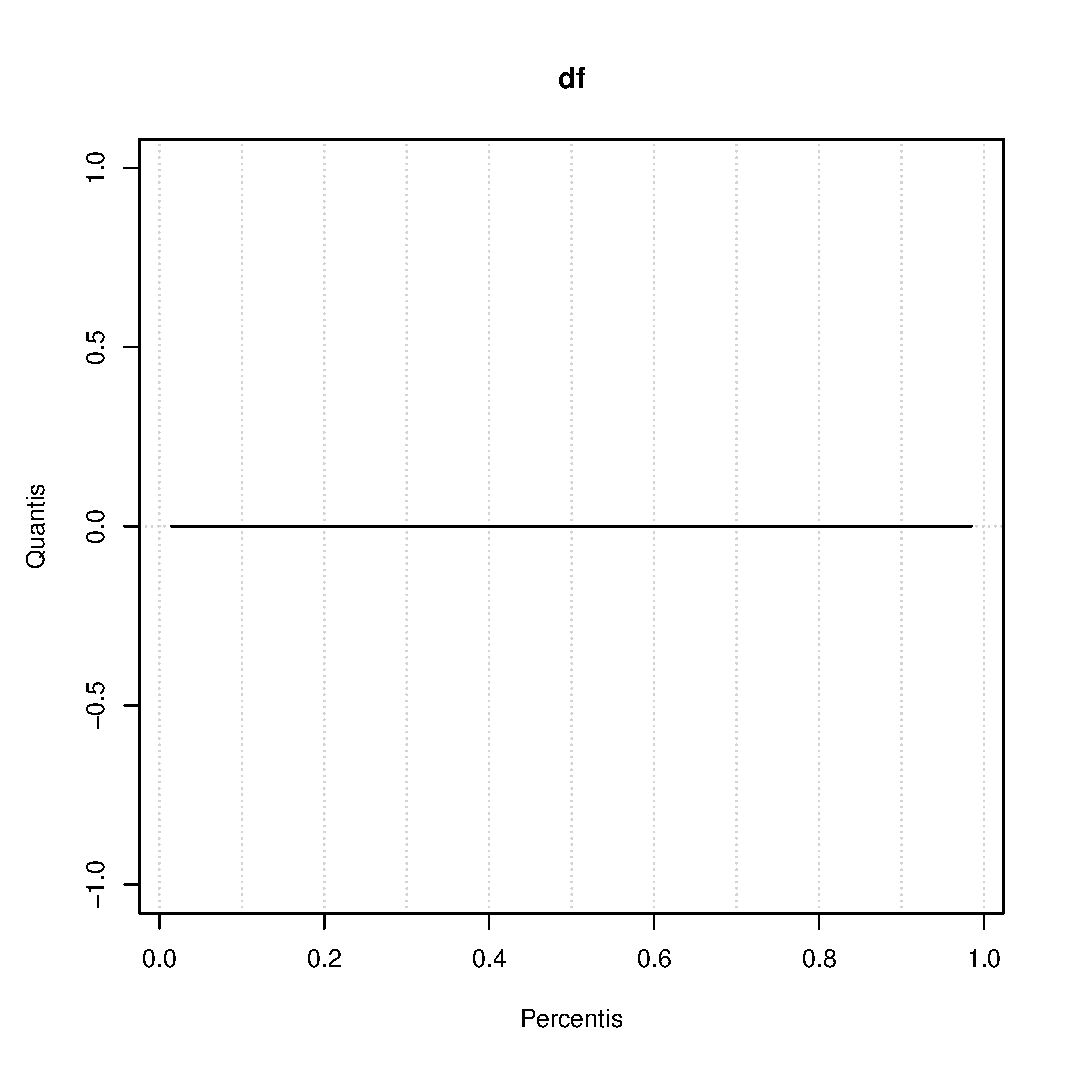
\includegraphics[width=0.6\textwidth]
      {dados/linux/df.eps}
  \caption{Gráfico de Percentis da métrica DF}
\end{figure}

\newpage

\begin{figure}[h]
  \centering
  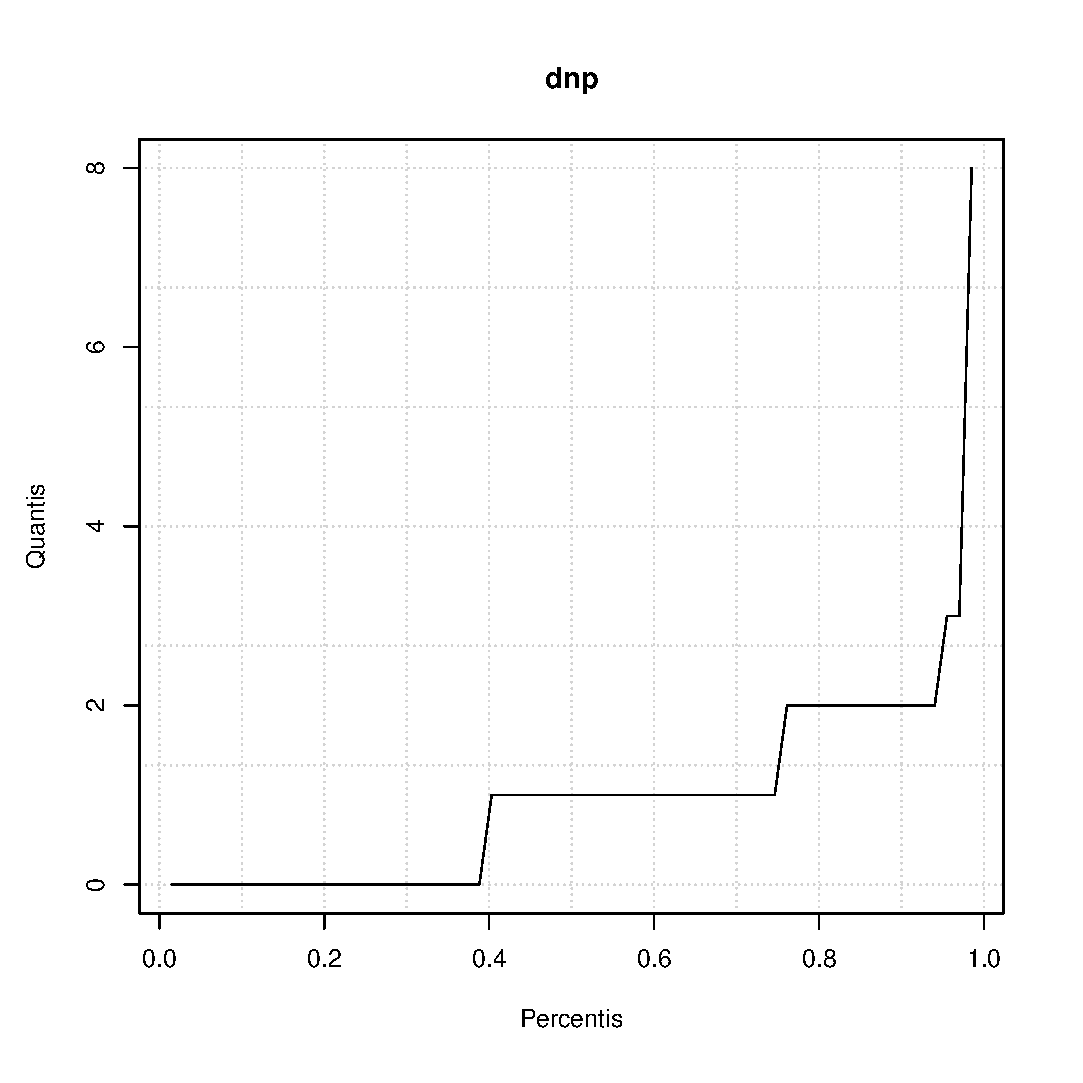
\includegraphics[width=0.6\textwidth]
      {dados/linux/dnp.eps}
  \caption{Gráfico de Percentis da métrica DNP}
\end{figure}

\begin{figure}[h]
  \centering
  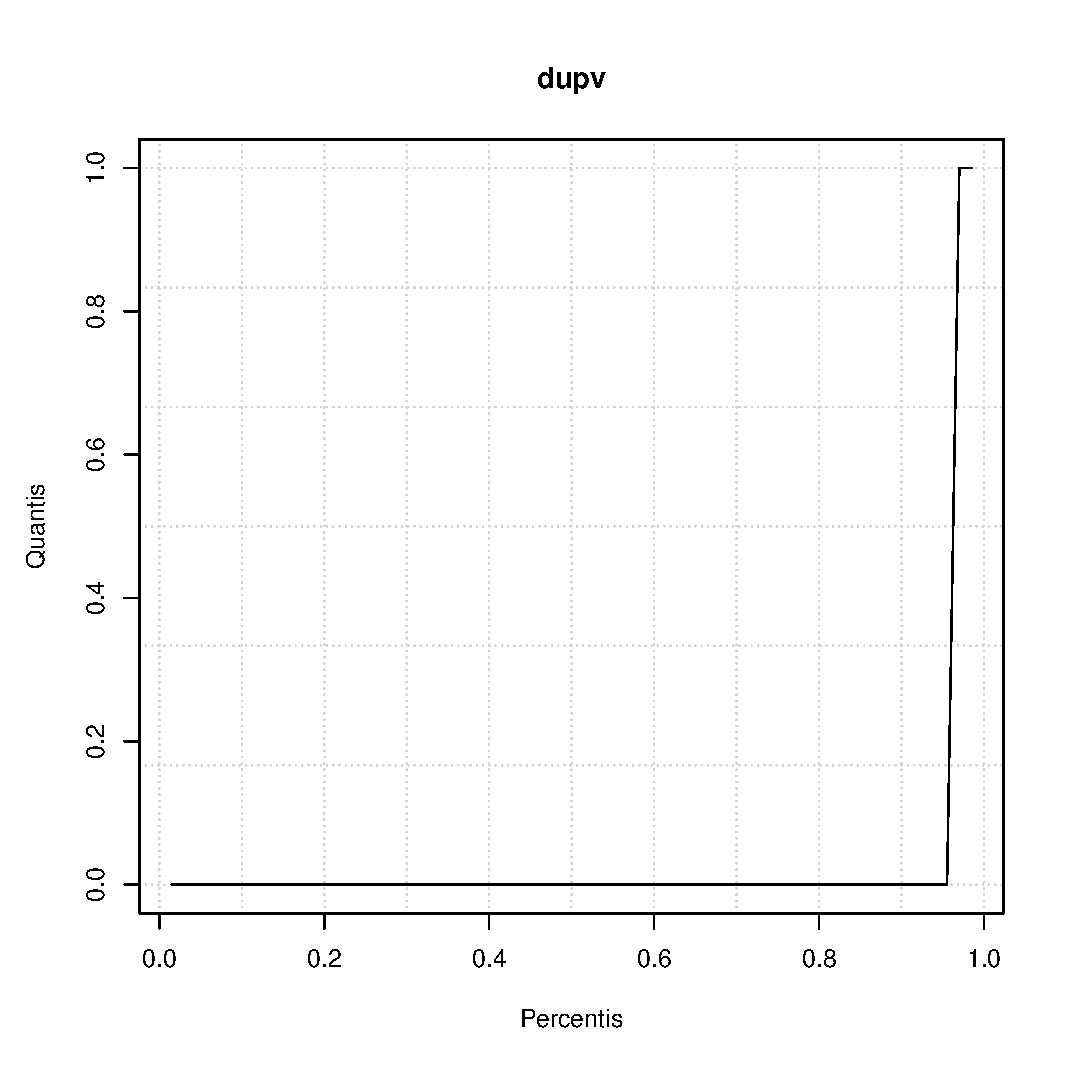
\includegraphics[width=0.6\textwidth]
      {dados/linux/dupv.eps}
  \caption{Gráfico de Percentis da métrica DUPV}
\end{figure}

\newpage

\begin{figure}[h]
  \centering
  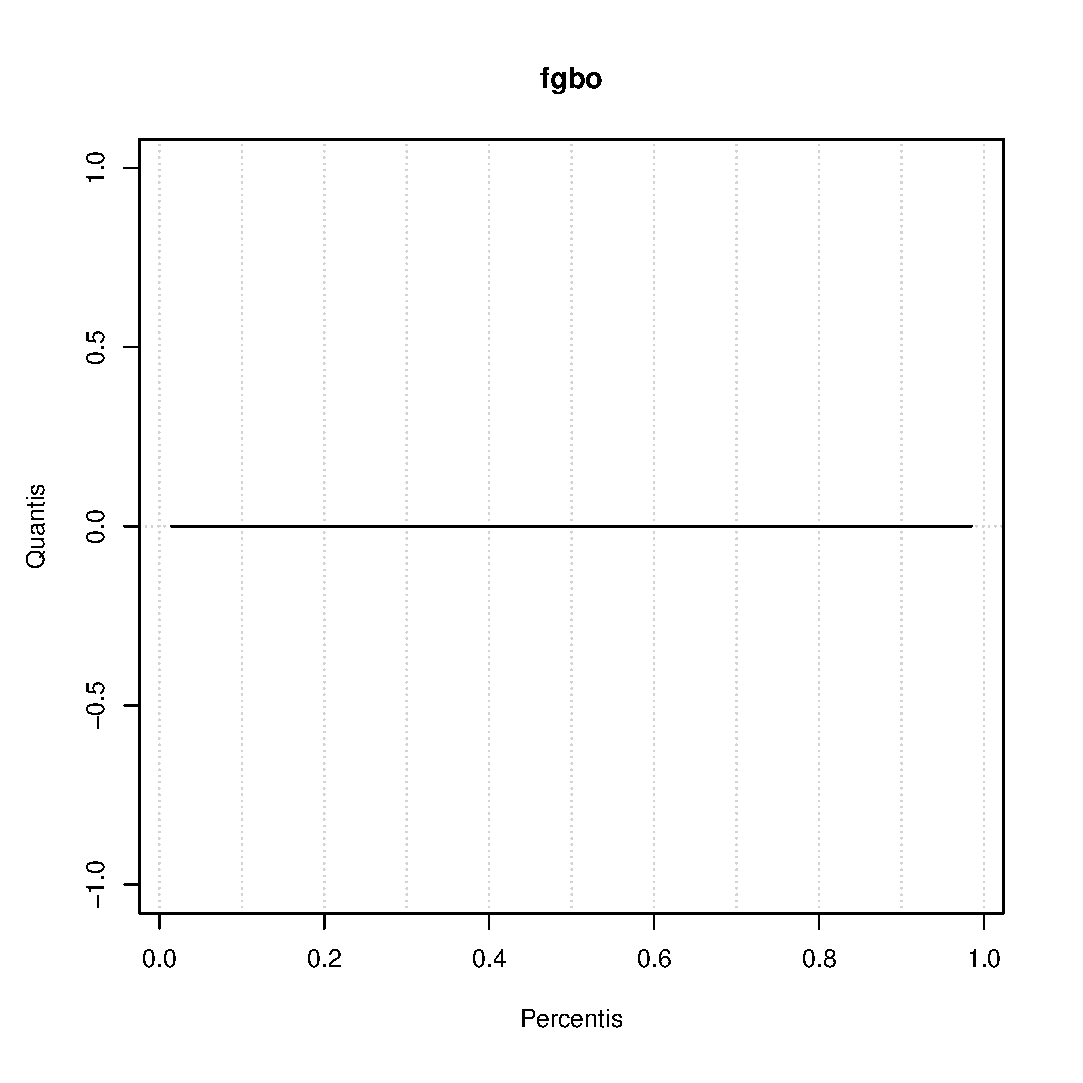
\includegraphics[width=0.6\textwidth]
      {dados/linux/fgbo.eps}
  \caption{Gráfico de Percentis da métrica FGBO}
\end{figure}

\begin{figure}[h]
  \centering
  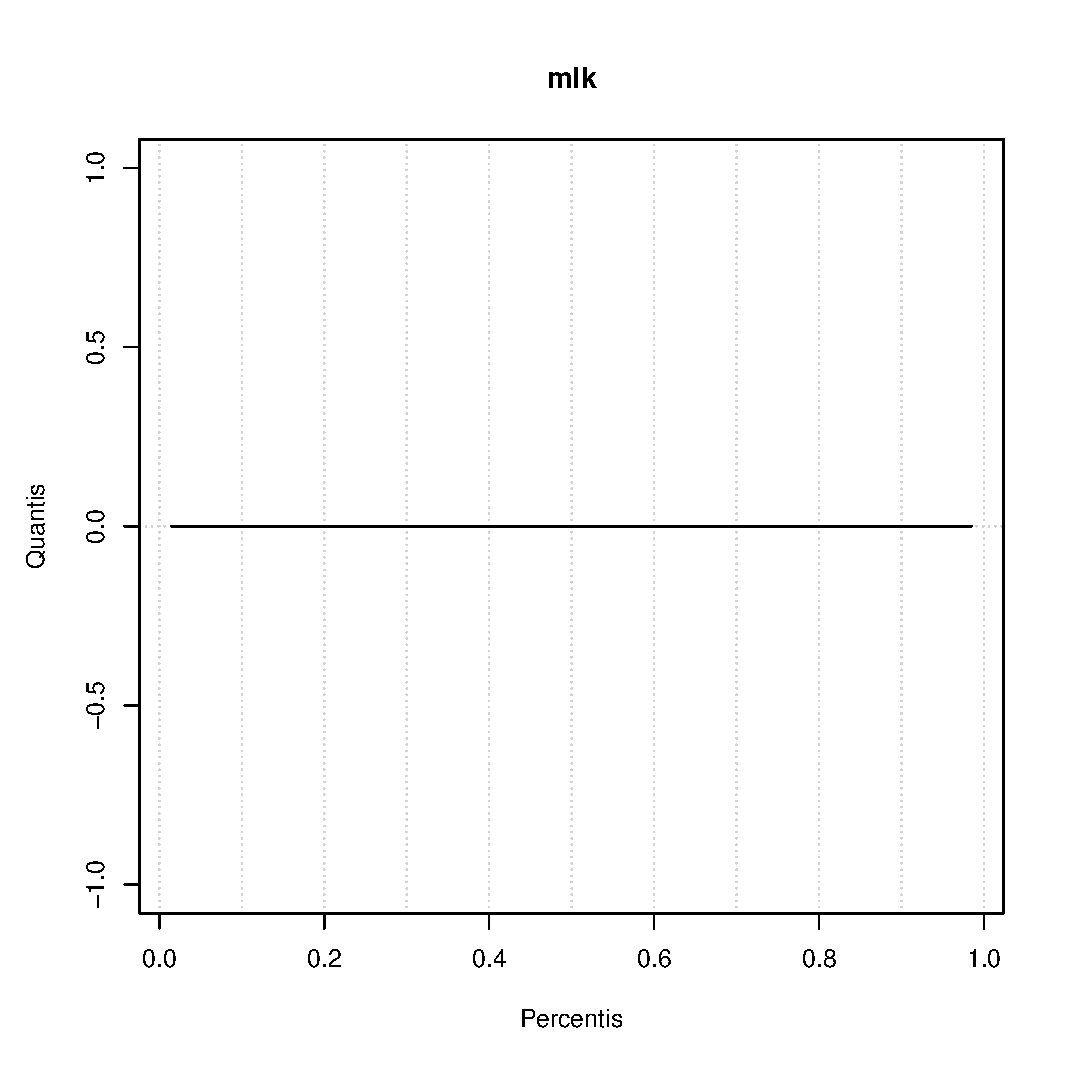
\includegraphics[width=0.6\textwidth]
      {dados/linux/mlk.eps}
  \caption{Gráfico de Percentis da métrica MLK}
\end{figure}

\newpage

\begin{figure}[h]
  \centering
  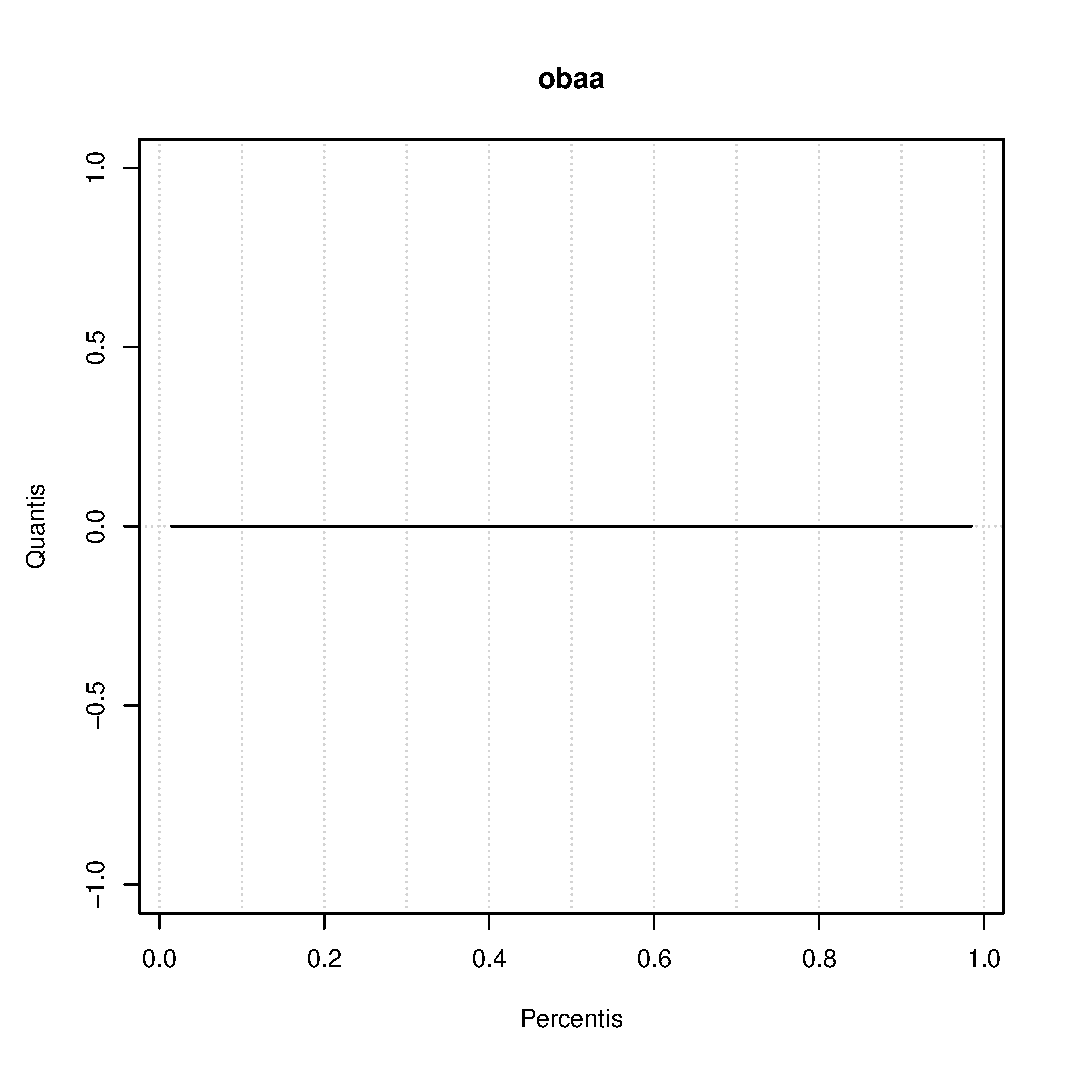
\includegraphics[width=0.6\textwidth]
      {dados/linux/obaa.eps}
  \caption{Gráfico de Percentis da métrica OBAA}
\end{figure}

\begin{figure}[h]
  \centering
  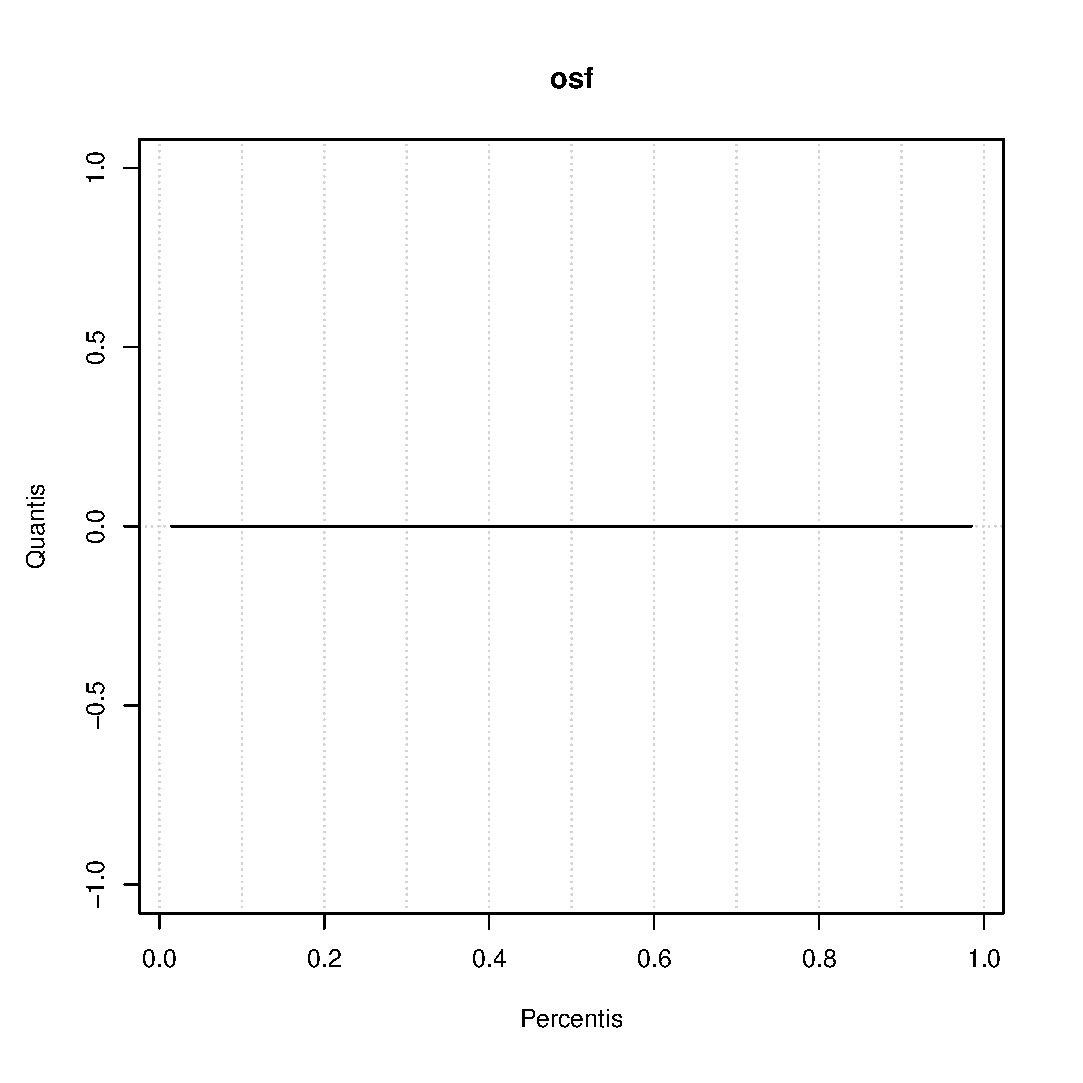
\includegraphics[width=0.6\textwidth]
      {dados/linux/osf.eps}
  \caption{Gráfico de Percentis da métrica OSF}
\end{figure}

\newpage

\begin{figure}[h]
  \centering
  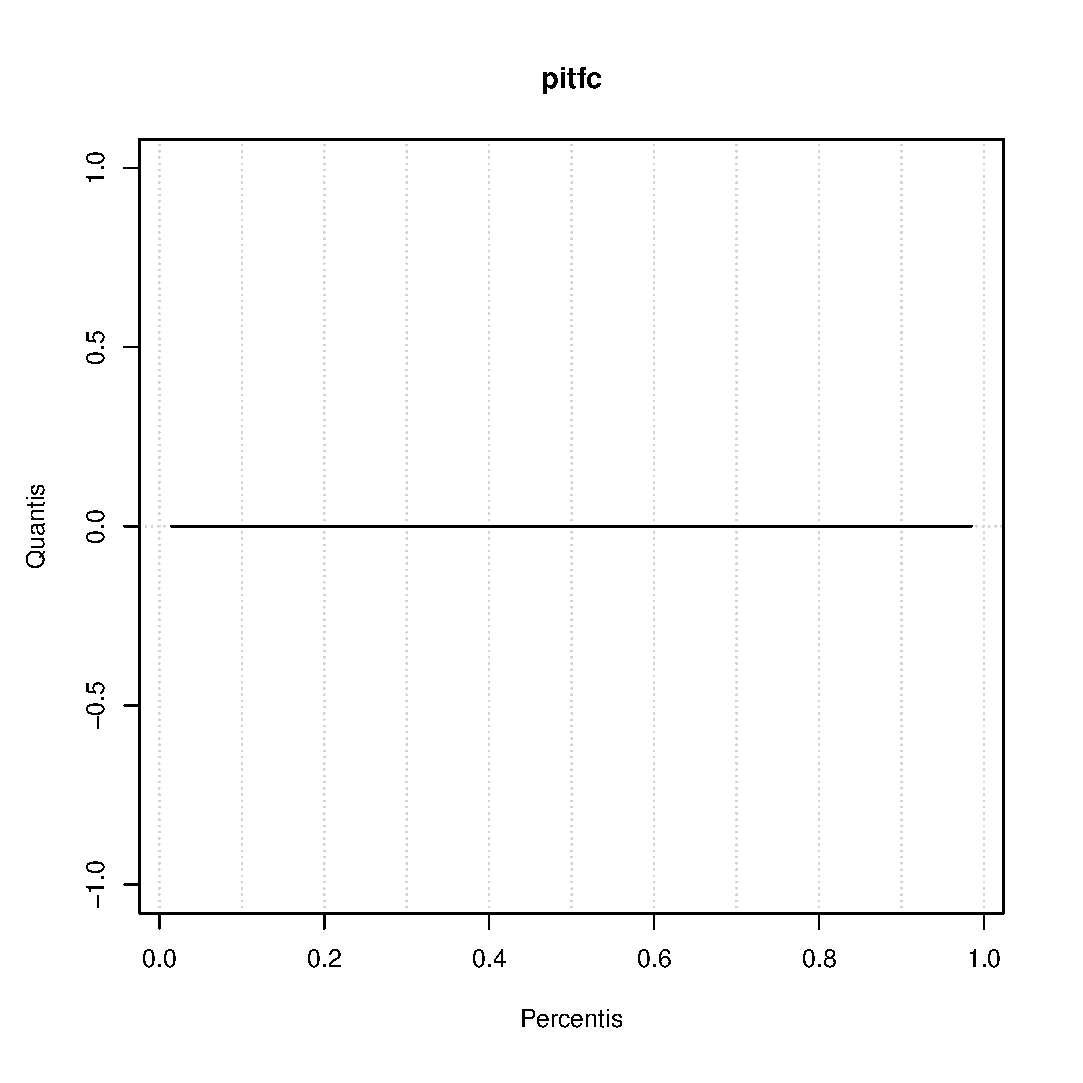
\includegraphics[width=0.6\textwidth]
      {dados/linux/pitfc.eps}
  \caption{Gráfico de Percentis da métrica PITFC}
\end{figure}

\begin{figure}[h]
  \centering
  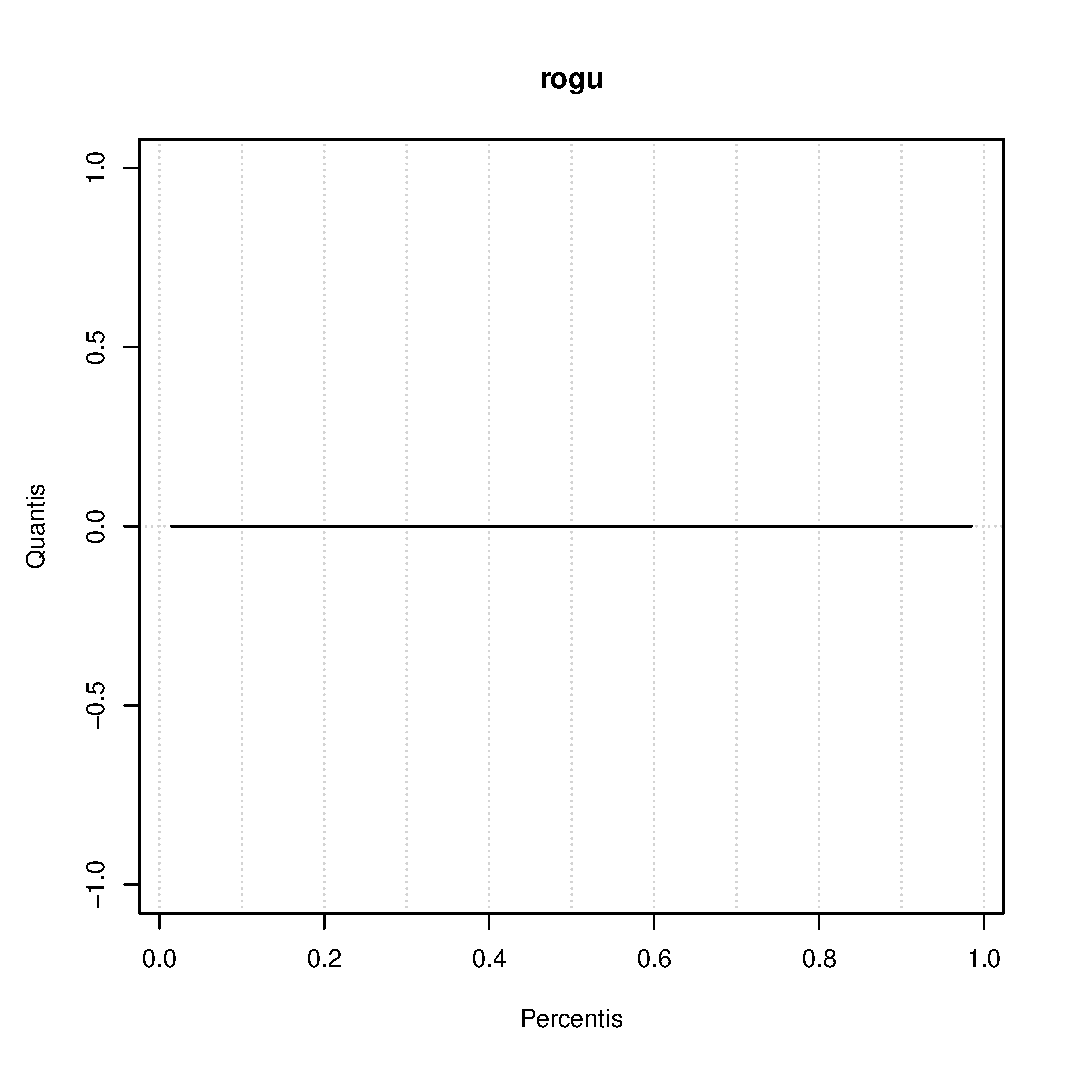
\includegraphics[width=0.6\textwidth]
      {dados/linux/rogu.eps}
  \caption{Gráfico de Percentis da métrica ROGU}
\end{figure}

\newpage

\begin{figure}[h]
  \centering
  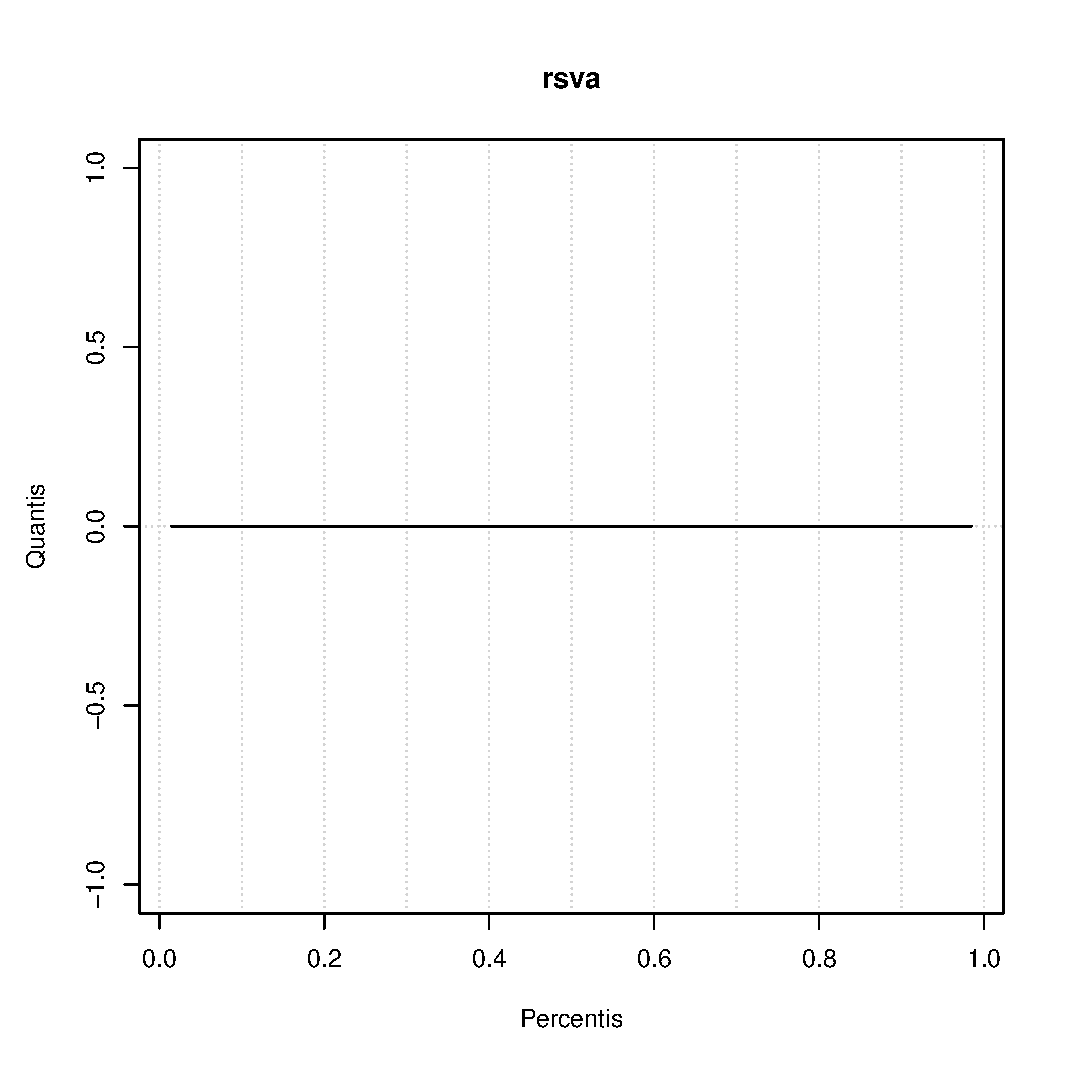
\includegraphics[width=0.6\textwidth]
      {dados/linux/rsva.eps}
  \caption{Gráfico de Percentis da métrica RSVA}
\end{figure}

\begin{figure}[h]
  \centering
  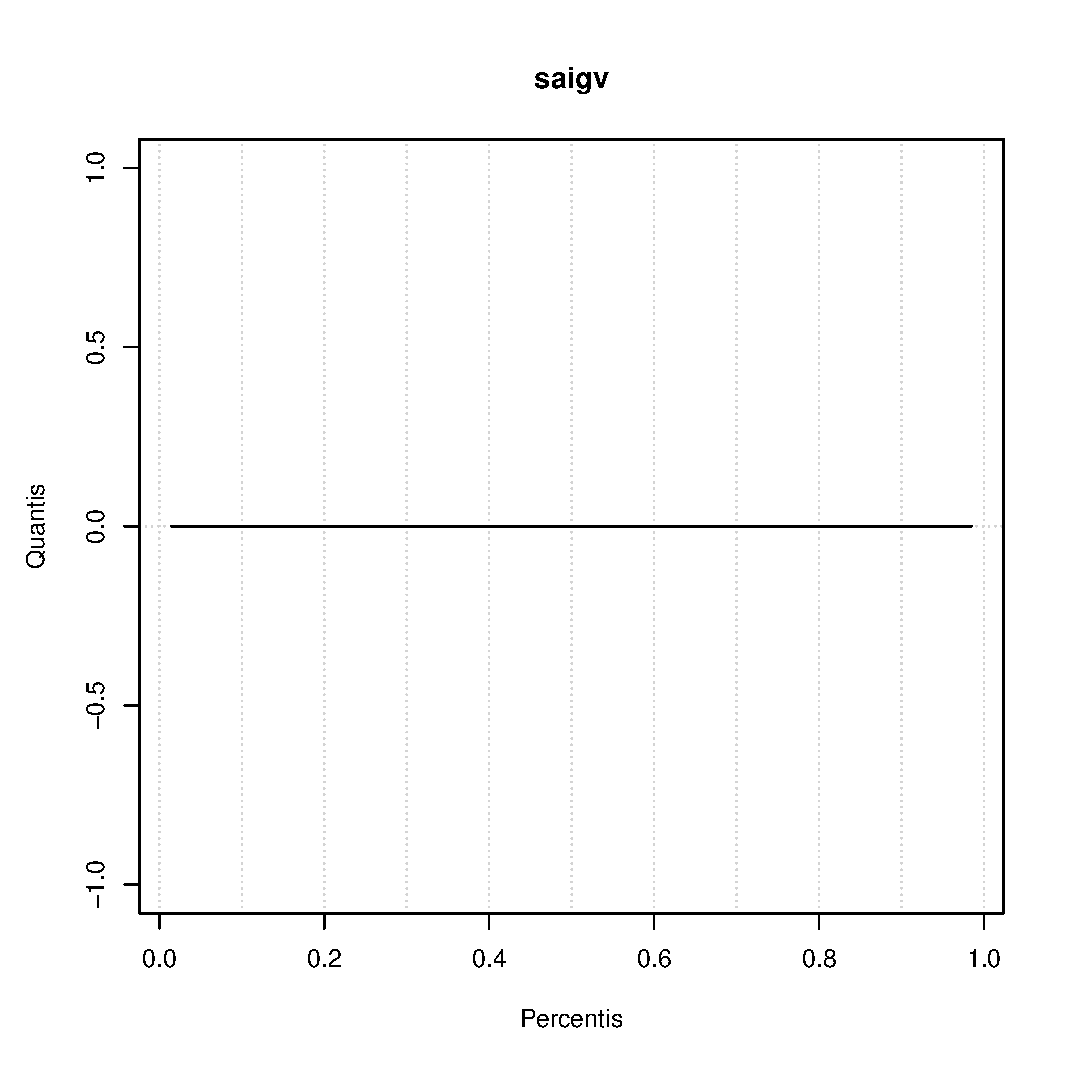
\includegraphics[width=0.6\textwidth]
      {dados/linux/saigv.eps}
  \caption{Gráfico de Percentis da métrica SAIGV}
\end{figure}

\newpage

\begin{figure}[h]
  \centering
  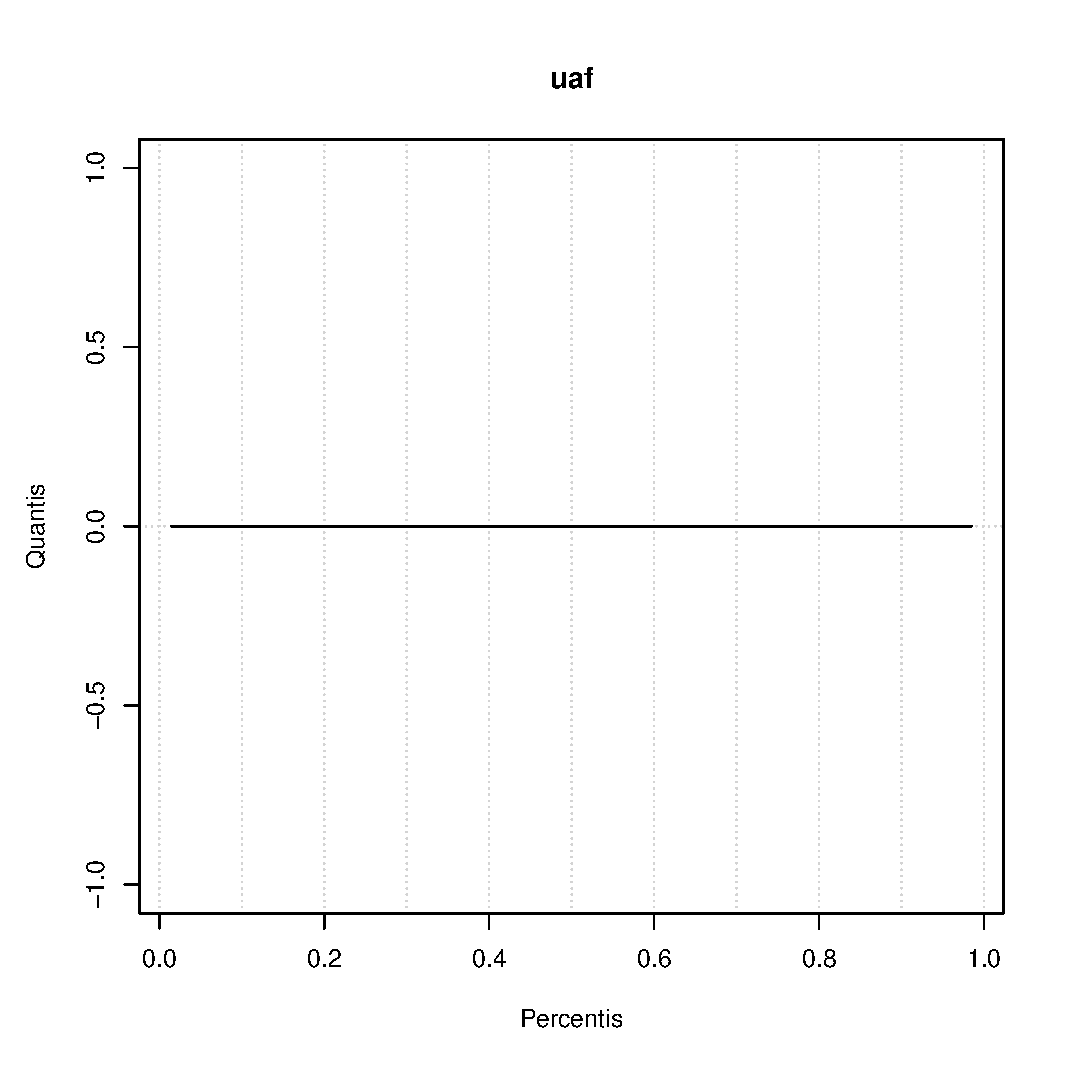
\includegraphics[width=0.6\textwidth]
      {dados/linux/uaf.eps}
  \caption{Gráfico de Percentis da métrica UAF}
\end{figure}

\begin{figure}[h]
  \centering
  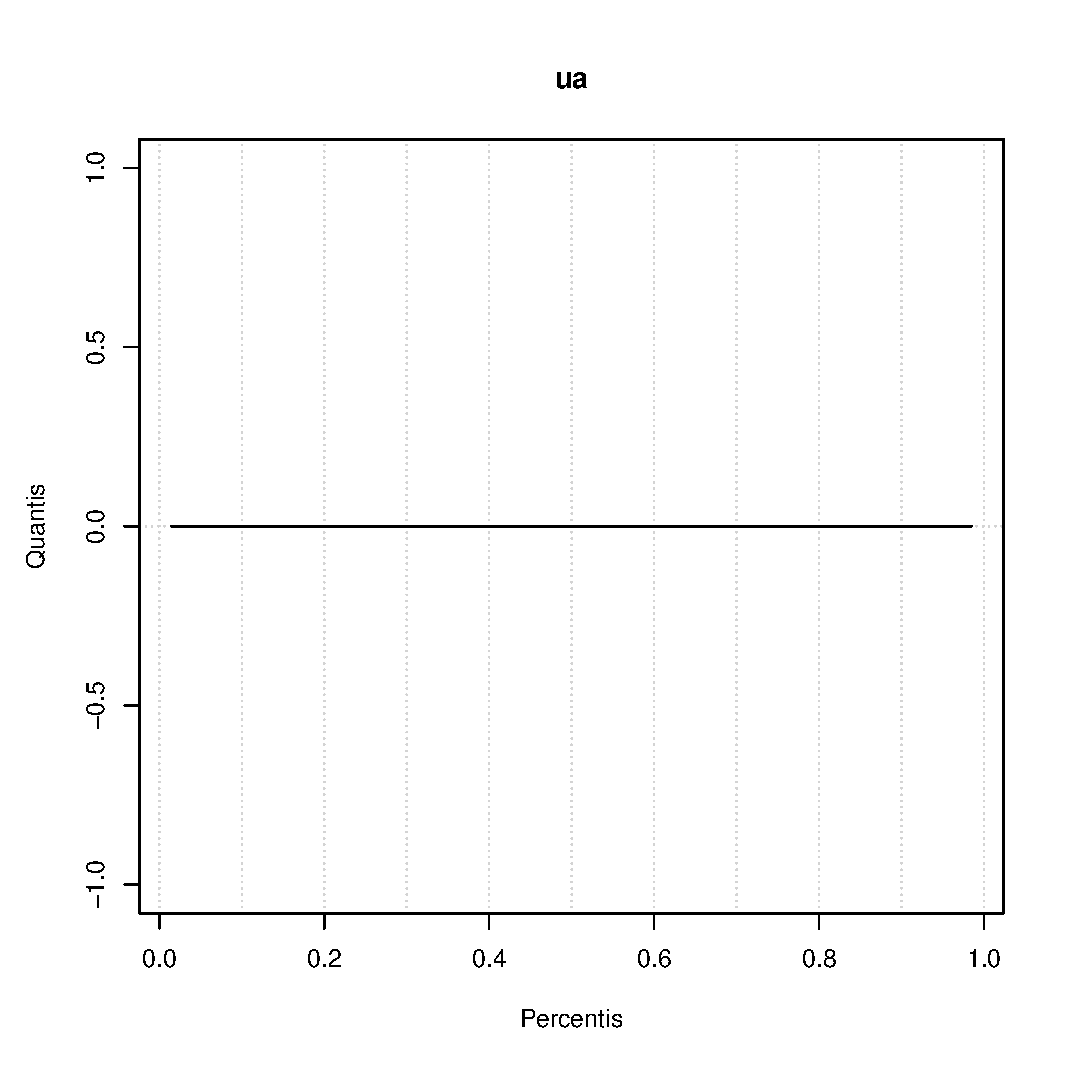
\includegraphics[width=0.6\textwidth]
      {dados/linux/ua.eps}
  \caption{Gráfico de Percentis da métrica UA}
\end{figure}

\newpage

\begin{figure}[h]
  \centering
  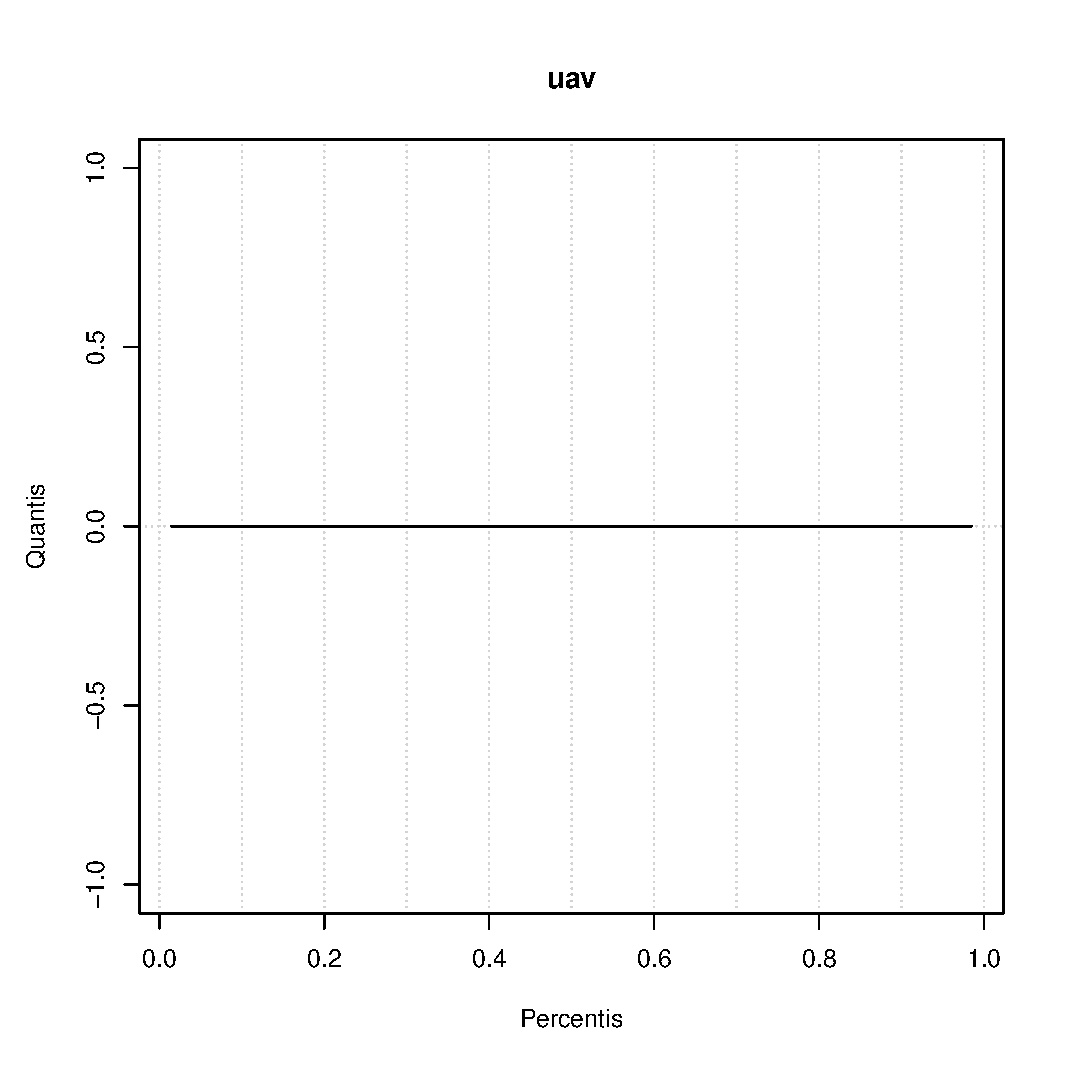
\includegraphics[width=0.6\textwidth]
      {dados/linux/uav.eps}
  \caption{Gráfico de Percentis da métrica UAV}
\end{figure}


\end{anexosenv}

